%\TEX root = ../../thesis_rui_almeida.tex


\section{DOAS}%
\label{sec:doas}

Differential Optical Absorption Spectroscopy is a well established
absorption technique that is widely used in the field of atmospheric
studies~\cite{Platt2007}. In this section, I present a short
introduction to the field, extracted from~\cite{ValentedeAlmeida2017},
an article we have published in 2017, marking the conclusion of the
initial studies for this PhD thesis.

There are two main families of \gls{DOAS} assemblies, with different
goals and capabilities:

\begin{itemize}

        \item Active systems, of which a simple illustration is
            presented in Fig.~\ref{fig:activeSmall}, are characterized
            by relying on an artificial light source for their
            measurements. A spectrometer at the end of the light path
            performs spectroscopic detection. Active DOAS techniques are
            very similar to traditional in-lab absorption spectroscopy
            techniques \cite{Platt2007};

        \item Passive DOAS techniques, illustrated in
            Fig.~\ref{fig:passiveSchematic}, use natural light sources,
            such as the Sun and the moon, in their measurement process.
            An optical system is pointed in certain elevation and
            azimuth angles and sends the captured light into a
            spectrometer, connected to a computer. The system returns
            the total value of the light absorption in its
            path~\cite{Platt2007,Merlaud2013}.

\end{itemize}

%f2
 \begin{figure*}[t]
    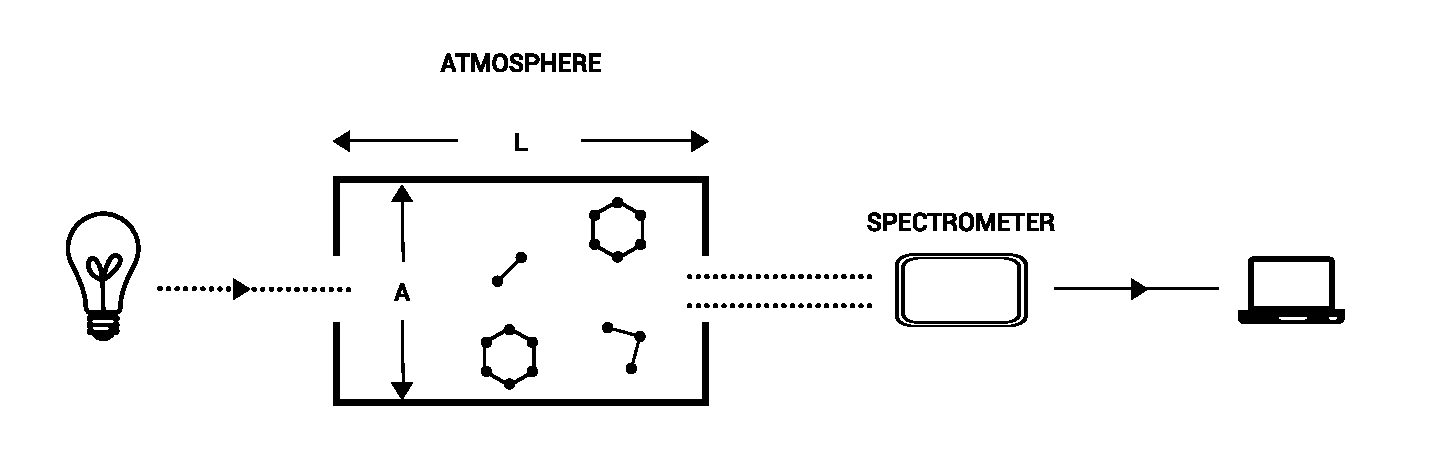
\includegraphics[width=14cm]{img/pdf/amt-2016-314-f02.pdf}
    \caption{Active DOAS schematic.}\label{fig:activeSmall}
  \end{figure*}

%f3
  \begin{figure*}[t]
      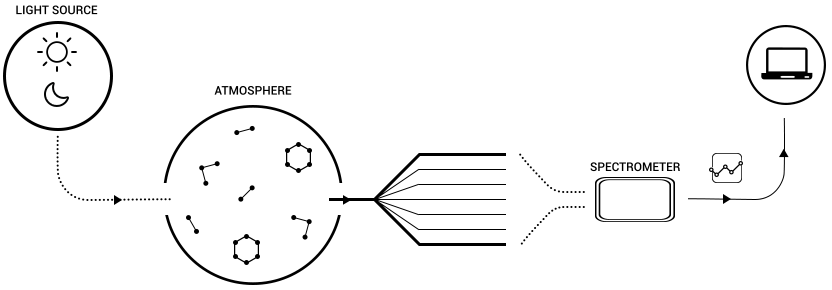
\includegraphics[width=14cm]{img/png/amt-2016-314-f03.png}
      \caption{Passive DOAS schematic.}\label{fig:passiveSchematic}
  \end{figure*}

DOAS itself is based on Lambert--Beer's law, which can be written as
\cite{Platt2007}

\begin{equation}
  \centering
  \label{eq:lambertBeer}
  I(\lambda) = I_0 (\lambda) \cdot \exp(-\sigma(\lambda) \cdot c \cdot L) \;,
\end{equation}

Where $\lambda$ is the wavelength of the emitted light; $I(\lambda)$ is
the light intensity as measured by the system; $I_{0}(\lambda)$ is the
intensity of the light as emitted by the source; and $\sigma(\lambda)$
is the absorption cross section of absorber, which is wavelength
dependent; $c$ is the concentration of the absorber we want to measure.


This law allows the definition of optical thickness
($\tau$)~\cite{Platt2007}:

\begin{equation}
      \label{eq:opticalThickness}
      \tau(\lambda) = \ln \bigg( \frac{I_{0}(\lambda)}{I(\lambda)}\bigg) = \sigma(\lambda) \cdot c \cdot
      L.
\end{equation}

In a laboratory setting, Eq.~(\ref{eq:lambertBeer})
or~(\ref{eq:opticalThickness}) can be used to directly calculate an
absorber's concentration, provided there is knowledge of  its cross
section. In the open atmosphere, however, absorption spectroscopy
techniques are far more complex. On one hand, $I_0(\lambda)$ is not
accessible since we measure from inside the medium we want to measure.
On the other hand, there are several environmental and instrumental
effects that influence measurement results. These effects include the
following~\cite{Platt2007}.

\begin{itemize}
      \item Rayleigh scattering is due to small molecules present in the
          atmosphere and is heavily influenced by wavelength (hence the
          blue colour of the
      sky).
      \item Mie scattering is caused by particles and larger molecules
          suspended in the atmosphere and is not very dependent
      on the wavelength (hence the white colour of clouds).
      \item Instrumental and turbulence effects are the instrument's
          transmissivity and atmospheric turbulence in the optical path
          also limit light intensity.

  \end{itemize}

In addition, we also have to take into account that, in the atmosphere,
there are a number of trace gases that interfere with passing light.

Another aspect worth mentioning is that our device is never pointed
directly at the light source (the Sun) but always processes light that
has been scattered at some unknown point in the optical path. This means
that the light that reaches our detector is only the scattered fraction
of the sunlight, depending on the system's position and geometry, as
well as wavelength.

The expansion of Lambert--Beer's equation to include all these effects
results in Eq.~(\ref{eq:expandedLambertBeer}).

\begin{align}
      \label{eq:expandedLambertBeer}
I(\lambda) & = I_{0}(\lambda) \cdot A(\lambda, \ldots) \cdot S(\lambda) \nonumber \\
      &\cdot
      \exp \Bigg[ - \int \Big[ \Big(\sum_{i} \sigma_{i}(\lambda, s) \cdot c_{i}(s)\Big) +
      \epsilon_\mathrm{M}(\lambda, s)\nonumber\\
      & + \epsilon_\mathrm{R}(\lambda, s) \Big]\mathrm{d}s \Bigg],
\end{align}

Where $A(\lambda, \ldots)$ is the fraction of scattered light that
reaches the device, $S(\lambda)$ represents instrumental and turbulence
effects, $\sigma_{i}(\lambda, s)$ is the absorption cross section of
absorber $i$, $c_{i}$ is the concentration of absorber $i$,
$\epsilon_\mathrm{R}(\lambda)$ represents Rayleigh's extinction
coefficient and $\epsilon_\mathrm{M}(\lambda)$ represents Mie's
extinction coefficient.


The interest of this equation lies within the retrieval of $c_i$, a
given absorber's concentration. Since the integral is taken along the
total atmospheric path of the measured photons, and considering that
their cross sections do not vary significantly in atmospheric
conditions, it is possible to define the concept of slant column, which
is of great importance~\cite{Merlaud2013}.

\begin{equation}
      \label{eq:slantColumn}
      \mathrm{SC}_{i} = \int c_{i}(s)\mathrm{d}s
\end{equation}

This quantity, as Eq.~(\ref{eq:slantColumn}) shows, equals the integral
of an individual absorber's concentration along the atmospheric optical
path of relevance.

Now, without knowledge of $I_{0}(\lambda)$, these equations cannot give
us absolute concentration values. We can, however, use another scattered
light spectrum as reference in Eq.~(\ref{eq:opticalThickness}). Instead
of absolute densities, this will yield relative changes in the
atmosphere. We thus arrive at Eq.~(\ref{eq:relativeOpticalThickness}).

\begin{align}
      \label{eq:relativeOpticalThickness}
      \ln\Big( \frac{I_\mathrm{ref}}{I}(\lambda) \Big) &= \ln\Big( \frac{A_\mathrm{ref}}{A}(\lambda,\ldots) \Big) + \ln\Big( \frac{S_\mathrm{ref}}{S}(\lambda) \Big) \nonumber\\
      &+  \sum_{i} (\sigma_{i}(\lambda) \cdot \Delta \mathrm{SC}_{i}(\lambda)) + \Delta \tau_\mathrm{M}(\lambda) \nonumber\\
      &+ \Delta \tau_\mathrm{R}(\lambda),
\end{align}

Where $\Delta \mathrm{SC}_{i}$  is the relative slant column of absorber
$i$; $\Delta \tau_\mathrm{M}$  is the relative Mie scattering term,
integrated to its optical thickness; and $\Delta \tau_\mathrm{R}$ is the
relative Rayleigh scattering term, integrated to its optical thickness.


This is where the principle of DOAS is applied. Instrument features,
scattering and other atmospheric effects have broad absorption spectral
profiles, which vary slowly with wavelength. Several trace absorbers
have narrow and rapidly varying spectral signatures in at least a small
section of the spectrum. By using Eq.~(\ref{eq:separation}), we can
separate these contributions \cite{Danckaert2015}.

\begin{equation}
      \label{eq:separation}
      \sigma(\lambda) = \sigma{'}(\lambda) + \sigma_{0}(\lambda)
\end{equation}

Here, the broad part of the optical thickness ($\sigma_{0}(\lambda)$)
can be separated from the narrow part ($\sigma{'}(\lambda)$ --
differential) by approximating it by a low-order polynomial, resulting
in Eq.~(\ref{eq:DOAS}).

\begin{equation}
      \label{eq:DOAS}
      \ln\Big( \frac{I_\mathrm{ref}}{I}(\lambda) \Big) = \sum_{i = 1}^{n} \sigma_{i}{'}(\lambda) \cdot \Delta \mathrm{SC}_{i} + \sum_{j = 0}^{m} a_{j} \cdot
      \lambda^{j},
\end{equation}

Where $\sum_{i = 1}^{n} \sigma_{i}{'}(\lambda) \cdot \Delta SC_{i}$ is
the differential part (narrowband, rapidly varying with wavelength) and
$\sum_{j = 0}^{m} a_{j} \cdot \lambda^{j}$ is a low-order polynomial,
used to remove the broadband spectral features resulting from
atmospheric and instrumental phenomena.


In practice, the mathematical solving of Eq.~(\ref{eq:DOAS}) is not
enough since it does not account for the Ring effect or the
non-linearities that result from stray light and wavelength shift in
measured and cross-section spectra.

The Ring effect is a consequence of rotational Raman scattering:
molecules in the atmosphere do not absorb photons in a purely elastic
(Rayleigh scattering) fashion. A small portion of the light--matter
interaction is in fact inelastic \cite{Brinkmann1968,Merlaud2013}. This
changes the light source frequencies as seen from the detector. This
phenomenon was first noticed by Grainger and Ring in 1962. At the time,
they noticed that the well-known Fraunhofer lines would slightly change
when one  observed them by using moonlight instead of scattered daylight
\cite{GRAINGER1962}.

From the occurrence of these phenomena, it results that the mathematical
procedure for DOAS measurements consists in solving a linear and a
non-linear problem. The linear problem is solved by writing
Eq.~(\ref{eq:DOAS}) in its matrix form:

\begin{equation}
      \label{eq:DOAS_matrix}
      \tau = \mathbf{A} \cdot X.
\end{equation}

$\mathbf{A}$ is an $m\,\times\,n$ matrix, with its columns being the
differential cross sections $\sigma_{i}{'}(\lambda)$ and the wavelength
powers taking the polynomial $P(\lambda) = \sum_{j = 0}^{m} a_{j} \cdot
\lambda^{j}$ into account. Since the number of lines in $A$ is much
larger than the number of columns, the system is overdetermined and, in
this case, we must use methods to numerically approximate a solution. It
is common to use the least-squares approach, in which the best solution
is the one that minimises $\chi^{2} = \left[\tau - A \cdot X\right]
\cdot \left[\tau - A \cdot X\right]^{T}$.

While the Ring effect is treated as a pseudo-absorber, a synthetically
produced~\cite{Chance1997} cross section that is fitted just like any
other absorber, non-linearities are addressed by applying
Levenberg--Marquardt's approach to non-linear fitting problems to
Eq.~(\ref{eq:DOAS_nonLinear}) \cite{Merlaud2013,Press2007}:


\begin{align}
      \label{eq:DOAS_nonLinear}
      &\ln\Big( \frac{I_\mathrm{ref}(\lambda)}{I(\lambda + \mathrm{shift}) + \mathrm{offset}} \Big) = \sum_{i = 1}^{n} \sigma_{i}{'}(\lambda) \cdot \Delta \mathrm{SC}_{i} \nonumber\\
      &+ \sum_{j = 0}^{m} a_{j} \cdot \lambda^{j},
\end{align}

Where shift and offset, which represent spectral wavelength shifts and
stray light offsets, respectively, are responsible for the non-linear
character of the problem.
